%!TEX root = main.tex

\chapter{Aplicaciones}
En esta sección se explicará a modo general el uso de la técnica propuesta y las potenciales aplicaciones que tienen los resultados obtenidos.
\section{Esquema de uso del algoritmo}
El esquema \ref{esq:PSO_ALG} resume el funcionamiento del algoritmo para el ajuste del modelo probabilístico a los datos del viento. A continuación se detallarán los pasos a seguir en el proceso de obtener el ajuste de parámetros de la distribución elegida.
\begin{enumerate}
    \item Lo primero que se realiza es el formateo de los datos, es decir, la conversión desde un conjunto de mediciones al formato utilizado por el programa desarrollado, en este caso se utiliza el \emph{comma-separated values} CSV. El \emph{script} utilizado dependerá del formato externo del cual provengan los datos.
    \item Una vez obtenidos los datos en el formato deseado, se procede a calcular las frecuencias de los registros obtenidos, para posteriormente ser comparadas con el modelo teórico. El número de frecuencias está determinado por la cantidad de subgrupos definidos que representan intervalos de datos.
    \item Antes de comenzar con el ajuste, se calcula una solución inicial ya sea de forma aleatoria (como es el caso para el ajuste de la velocidad del viento) o mediante algún método conveniente (como la aproximación numérica para el caso del ajuste de la dirección del viento).  
    \item Definiendo la cantidad de partículas y el número de iteraciones, se ejecuta el algoritmo \emph{Particle Swarm Optimization} para que mejore la estimación inicial de acuerdo a una función objetivo previamente definida. 
    \item Finalmente, una vez que el algoritmo termina, entrega los valores de los parámetros para la función de densidad de probabilidad (fdp) elegida. En esta memoria se utilizaron la distribución de Weibull y la \emph{mixture of von Mises distribution}. Con ello, es posible elaborar un histograma y graficar la fdp para evaluar el ajuste obtenido.
\end{enumerate}
En meteorología, la velocidad del viento se registra en nudos por segundo, pero en esta memoria se convirtieron los datos de acuerdo al sistema internacional SI, o sea, a metros por segundo. La conversión consta en multiplicar el valor de los nudos/segundo por 0.514444 para obtener los metros/segundo correspondientes, como se describe en el libro de unidades internacionales de medidas de la Universidad de Illinois \cite{KnotsMeterSeconds}.\\
El sistema de referencia utilizado para la interpretación de los datos de dirección del viento es el conocido como la rosa de los vientos \cite{RosaViento}. Dicho sistema ubica el Norte en el grado 0, al Este en el grado 90, al Sur en el grado 180 y al Oeste en el grado 270, siendo la dirección determinada el origen desde donde proviene el viento. Ejemplo, si la dirección predominante del viento en cierto intervalo de tiempo es de 90 grados, entonces diremos que la corriente de viento proviene desde el este.

\begin{figure}[ht!]
\caption{Esquema de uso del algoritmo}
% Define block styles
\tikzstyle{decision} = [diamond, draw, fill=blue!20, 
    text width=4.5em, text badly centered, node distance=3cm, inner sep=0pt]
\tikzstyle{block} = [rectangle, draw, fill=blue!20, 
    text width=15em, text centered, rounded corners, minimum height=4em]
\tikzstyle{blockALG} = [rectangle, draw, fill=green!20, 
    text width=15em, text centered, rounded corners, minimum height=4em]
\tikzstyle{line} = [draw, -latex']
\tikzstyle{cloud} = [draw, ellipse,fill=red!20, node distance=7cm,
    minimum height=2em]
    
\begin{tikzpicture}[node distance = 3cm, auto]
    % Place nodes
    \node [block] (dataFormat) {Ajuste formato de los datos};
    \node [cloud, left of=dataFormat] (inputData) {Datos};
    %\node [cloud, right of=init] (system) {system};
    \node [blockALG, below of=dataFormat] (initAlg) {Cálculo de frecuencias, por rango (continuas) o discretas};
    \node [blockALG, below of=initAlg] (SolIni) {Estimación inicial de parámetros};
    \node [blockALG, below of=SolIni] (PSO) {PSO ajusta los parámetros de la fdp};
    \node [block, below of=PSO, node distance=3cm] (grafico) {Visualización del ajuste con histograma y fdp};
    % Draw edges
  
    \path [line] (dataFormat) -- node {\footnotesize{\emph{CSV con datos formateados}}}(initAlg);
    \path [line] (initAlg) -- node {\footnotesize{\emph{Fecuencias calculadas, parámtros}}}(SolIni);
    \path [line] (SolIni) -- node {\footnotesize{\emph{Estimación inicial}}}(PSO);
    \path [line] (PSO) -- node {\footnotesize{\emph{Vector de parámetros}}}(grafico);
    \path [line,dashed] (inputData) -- (dataFormat);
\end{tikzpicture}

\label{esq:PSO_ALG}
\end{figure}

\section{Uso de los resultados}
En la siguiente sección se describirán algunas de las potenciales aplicaciones de los resultados que se obtienen al utilizar las técnicas propuestas en esta memoria.
\subsection{Energía eólica}
En el ámbito de la energía eólica, como se expone en Dabbaghiyan et al. \cite{Dabbaghiyan15}, Farade \cite{Fadare08}, Weisser \cite{Weisser02}, Masseran et al. \cite{Winddirelse15}, Shata et al. \cite{Shata05} y Carneiro et al. \cite{Carneiro15}, la determinación del potencial eléctrico del viento en una región es fundamental al momento de determinar la viabilidad de un proyecto de generación de energías renovables. Así mismo, saber cuáles son las direcciones del viento predominantes en una zona ayudará a determinar el mejor emplazamiento posible para una planta de generación de energía eólica.\\
El Dr. Samir Kouro, ingeniero civil electrónico de la Universidad Técnica Federico Santa María, explica desde la perspectiva del tema tratado en esta memoria los aspectos a considerar al momento de evaluar un proyecto de energía eólica:
\begin{enumerate}
  \item La distribución de Weibull permite obtener información acerca de la magnitudes promedio alcanzadas por la velocidad del viento en un determinado rango de tiempo. De esta forma, se puede evaluar el potencial eléctrico de una región con el fin de determinar la factibilidad de un proyecto eólico. Así mismo, los valores extremos de la distribución de Weibull, en particular los valores máximos, ayudan a determinar las características de las turbinas a implementar, es decir, la resistencia de las torres que sostienen las hélices y la forma de las mismas, para que estas sean resistentes a las fuertes corrientes de viento.\\ 
  La Figura \ref{fig:ejemplo_potencial}, muestra las zonas importantes a considerar acerca del comportamiento de la velocidad del viento.
  \item El modelo para la dirección del viento permite determinar las direcciones predominantes de manera de establecer los lugares en donde se ubicaran las turbinas de viento. Un mal emplazamiento de estas implica una disminución en el rendimiento de las turbinas y un desaprovechamiento de la energía obtenida desde el viento.\\
  La figura \ref{fig:ejemplo_emplazamiento} muestra un esquema de emplazamiento de turbinas para aprovechar la dirección del viento.\\
\end{enumerate}
\begin{figure}[ht!]
    \centering
    \captionsetup{justification=centering,margin=2cm}
        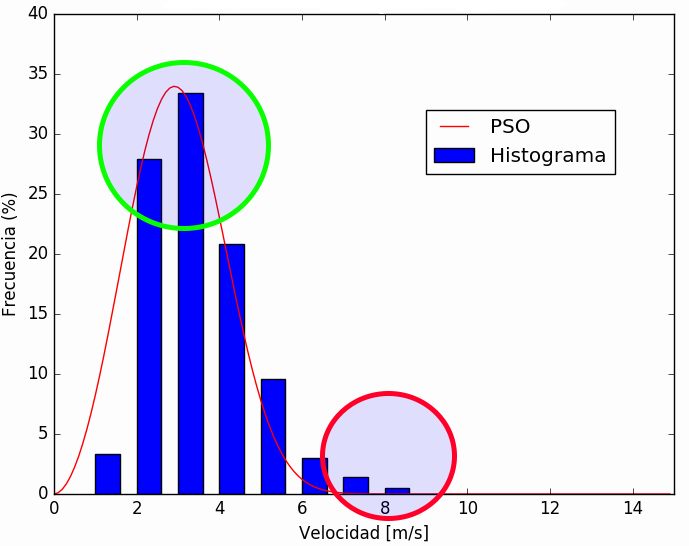
\includegraphics[width=0.8\textwidth]{figures/result_2014_ejemplo_potencial.png}  
    \caption{Ejemplo de zonas a evaluar en la velocidad del viento.\\ Fuente: Elaboración propia.}
    \label{fig:ejemplo_potencial}
\end{figure}

\begin{figure}[ht!]
    \centering
    \captionsetup{justification=centering,margin=2cm}
        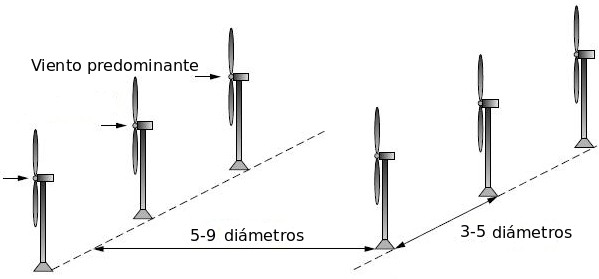
\includegraphics[width=0.8\textwidth]{figures/ejemplo_emplazamiento.jpg}  
    \caption{Ejemplo emplazamiento turbinas eólicas.\\ Fuente: Jorge Mírez \cite{figureEmplacement}.}
    \label{fig:ejemplo_emplazamiento}
\end{figure}
%En el trabajo de Shata et al. \cite{Shata05}, se menciona que el rango de generación eléctrica para el viento es entre los 5 y 6 metros por segundo. Por lo observado en la sección de resultados 
\subsection{Propagación de incendios}
Los incendios son una problemática que muchos lugares del mundo deben combatir debido a diversos factores que los provocan, ya sean de origen natural, debido a las condiciones climáticas, por errores humanos, entre otros. En particular, el grave incendio ocurrido en Valparaíso el mes de abril del año 2014 \cite{incendioValpo} que provocó severos daños a la ciudad, es una muestra de la influencia que tienen las condiciones del clima en la propagación de los incendios. Como se destaca en el artículo \cite{incendioValpo} las altas temperaturas y los fuertes vientos son un factor negativo que ayuda a los incendios a expandirse y revivir focos parcialmente extinguidos.\\
En el trabajo de Beer \cite{Beer91}, se expone la relación entre el fuego y los vientos, explicando por ejemplo el cómo influye la velocidad de los vientos en la propagación de las llamas.\\
Las cifras que se obtienen de los modelos obtenidos en esta memoria permiten realizar una estimación inicial del comportamiento del viento en, por ejemplo, las fechas recurrentes de incendios forestales, de forma tal que se pueda realizar un plan estratégico que permita abordar estos incidentes de manera más eficiente, disminuyendo el impacto en las zonas afectadas.

\subsection{Propagación de pesticidas}
En el área de la agricultura, la volatilización representa la mayor forma de disipación de pesticidas aplicadas a suelos o cultivos. Como se explica en el trabajo de Bedos et al. \cite{Bedos01}, generalmente la volatilización de los pesticidas (ver Figura \ref{fig:ejemplo_pesticidas}) en un proceso que dura varias semanas, por lo que es necesario tener un control sobre las variables que inciden en este proceso. Entre los factores atmosféricos, la velocidad del viento tiene una directa incidencia en la razón de volatilización de los pesticidas.\\
La distribución de Weibull, puede proveer de información relativa a las velocidades de viento predominantes y así ayudar a planificar la aplicación de pesticidas en los cultivos.
\begin{figure}[ht!]
    \centering
    \captionsetup{justification=centering,margin=2cm}
        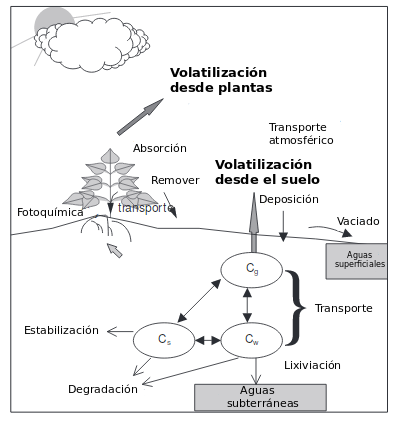
\includegraphics[width=0.8\textwidth]{figures/pesticide_wind.png} 
    \caption{Principales procesos que interactúan en el comportamiento de los pesticidas después de su aplicación.\\ Fuente: Bedos \cite{Bedos01}.}
    \label{fig:ejemplo_pesticidas}
    
\end{figure}

\subsection{Análisis atmosférico}
En el estudio realizado por García-Portugués et al. \cite{Portugues12}, se propone un método para explorar la relación entre la dirección del viento y las concentraciones atmosféricas de SO$_2$ monitoreadas en una estación cercana a una planta de energía en la región de Galicia, España, con el fin de comparar la eficiencia de las medidas de precaución implementadas en ese país para la reducción de la contaminación. Las técnicas propuesta en esta memoria, pueden utilizarse para el modelamiento de la dirección del viento, de manera de 
aportar información relevante al comportamiento de elementos contaminantes en la atmósfera.

\subsection{Resumen del capítulo}
Los métodos propuestos en esta memoria entregan información teórica basada en datos históricos acerca de la velocidad y la dirección del viento. Dicha información puede ser utilizada principalmente para la evaluación de la factibilidad de distintos proyectos afines. En otros casos, permite realizar un estudio pertinente a las condiciones climáticas, en las que el viento es un factor determinante en el comportamiento del entorno.